\section{Results}\label{results}
% Notes about conditions where worse performance is observed with FFL:
% * The issues are documented in the study notes but the biggest point seems to be that people have trouble recalling syntax even if they have no issues practicing during the tutorial and have to spend good amount of time reading through the cheat sheet again, especially if they were using LaTeX for the first task with a gap between  the task and the tutorial. This is not the case with LaTeX. The also explains why B is worse than A.
% * The other major sticking point is that people would frequently get stuck on a typo or semicolon for 2min+ since our error message doesn't tell them where it is

In this section, we describe our findings. Participants are referred to by pseudonyms \textit{P1--33}. P1--28 were included in our quantitative tests and results. P32--33 completed a variant of the study that involved use of a personal laptop. To convey representativeness of the findings, observations are accompanied with numbers indicating how many participants an observation reflects (e.g., ``(5)'' means 5 participants).

\subsection{Effect of FFL on task success} % Zed: changed to title case

Overall, there was significant improvement in task time, self-reported ease, and readability when participants used FFL for editing tasks (E1 \& 2), and no perceived difference for creation tasks (C1 \& 2).

\subsubsection{Completion rate} Overall, participants completed tasks at about the same rate when using FFL and LaTeX. Most participants succeeded in most tasks: altogether, participants reached the time limit on less than 20\% of tasks, amounting to 6 failed FFL tasks and 12 failed LaTeX tasks. The most difficult task for LaTeX seemed to be task E2 where 8 participants failed to complete in the LaTeX condition ($p=0.025$, {Fisher's Exact Test}~\cite{fisher}).
When asked to indicate the extent to which they were able to do what they wanted on a 7-point Likert scale (Figure \ref{fig:responses}), there was no significant difference between FFL and LaTeX ($F=0.792$, $p=0.565$).
A complete listing of per-task completion rates appears below in \hyperref[tab:count_fail_task]{Table~\ref{tab:count_fail_task}}.

% \subsubsection{``I was able to do what I wanted with the tool.'' (1-7)}\ \\[1ex]
% \scalebox{0.93}{
%     \begin{tabular}{l|r r r r r}
%         Avg. Score (1-7) & Task A & Task B & Task C & Task D & Open Task \\\hline
%         FFL     &6.06&5.69&6.63&5.44&6.30\\
%         \LaTeX  &6.00&6.29&5.88&4.72&N/A
%     \end{tabular}
% }\\[1ex]
% From Table \ref{tab: was_able_table} in \ref{sec: result_table}, we see no significant difference between the participants' response to the statement, regardless of grouping. We suspect this is due to most participants being able to complete the tasks or come close to doing so.

% \andrew{We need to compute a non-inferiority test to make the claim for ``at least as well''---see Sec 6.1.5 in \url{https://drive.google.com/file/d/1clTJm6CZIpvFzpAumCRg1ehiWdVGpY1X/view?usp=share_link}}

% In general, participants were able to complete the tasks within the allotted time, with only a small handful of participants reaching the time limit (see Table \ref{tab: count_fail_task} in the \ref{sec: result_table}).
% \andrew{Let's replace these tables (in all the sections) with prose. If we keep these tables (which I'm not sure if we should) then let's put them in the appendix.}
% \begin{center}
%     \begin{tabular}{l|r r r r}
%         & Task A & Task B & Task C & Task D \\\hline
%         FFL     &3&2&0&1\\
%         \LaTeX  &2&1&1&8
%     \end{tabular}
% \end{center}
% Less than 10 \% of participants were not able to complete any given task within the time limit, with the exception of those using \LaTeX\ on task D; 8 participants were not able to complete this task in time. We see that in the simple tasks (A \& B), more participants were not able to complete the tasks using FFL compared to \LaTeX. Although this might be an statistically insignificant amount and we do not observe a significant learning effect in later statistics, we do note similar trends in a few other metrics, and we discuss potential potential reasons for this in \ref{qualitative_analysis}. In contrast, FFL performed significantly better in tasks C \& D. This difference is also reflected in most of the other metrics we have measured.
% hita - can you add what metrics you're referring to in this phrase: "we do note similar trends in a few other metrics"

\subsubsection{Speed}

\begin{figure}
    \centering
    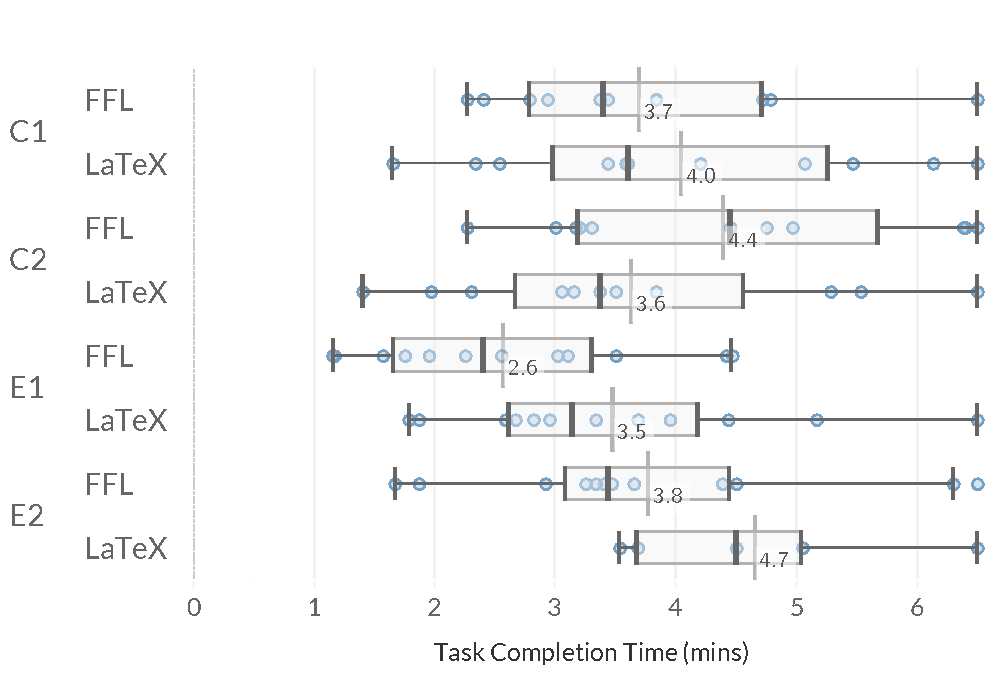
\includegraphics[width=\linewidth]{figures/Timing.pdf}
    \caption{Task completion time. Participants completed tasks E1 \& 2 significantly faster with FFL than with LaTeX. \normalfont Box-and-whiskers depict median, quartiles, and extrema (within 1.5 IQR). An additional, taller vertical line annotates the average. Individual times are rendered as dots in the background. Incompletes are encoded as maximum time. \zed{Per-row mean time and standard deviation appear in \hyperref[tab:speed_table]{Table \ref{tab:speed_table}}.}}
    \Description{Boxplot showing completion times by task and interface. The median completion time is lower with FFL than LaTeX for tasks C1, E1, and E2; and higher for task C2. Tasks C1 and C2 see greater variance in task completion time regardless of interface. For tasks E1 and E2, the median, average, minimum and maximum time are shorter with FFL than LaTeX.}
    \label{fig:timing}
\end{figure}

As depicted in \hyperref[fig:timing]{Figure~\ref{fig:timing}}, participants completed the complex editing tasks (E1 \& E2) more quickly with FFL than with LaTeX. A linear mixed-effects model found the interface to have a significant effect ($F=6.7$, $p=0.02$). Other significant effects include task ($F=11$, $p=2\times10^{-5}$) and task-interface interaction ($F=6.8$, $p=0.001$); task order was not significant. As implied by the task-interface interaction effect, the effect of FFL was stronger for some tasks than others. Fitting the same model to the pairs of creation (C1 \& 2) and editing (E1 \& 2) tasks separately, the effect of FFL was significant for editing tasks ($F = 27$, $p=7\times10^{-5}$), but not for the creation tasks ($p\approx1$). 
\zed{While these test statistics are in part affected by our choice to cut off participants at 6.5 minutes, a visual inspection suggests the trends hold for participants who were not cut off: FFL decreased task time for the 0th--75th quartiles, ranges for which no participants had reached the cutoff limit (see Figure~\ref{fig:timing}). Our observations of participants revealed no clear indications that participants were further from complete when cut off in the FFL condition than in the baseline condition.}
% \zed{Note that participants were instructed to terminate their task at 6.5 minutes regardless of completion, although the median and quartiles in \hyperref[fig:timing]{Figure~\ref{fig:timing}} should still give an impression of the distributions otherwise. Many participants who reached the time limit were ``stuck'' on singular issues, the reasons for which we will discuss in Section~\ref{sec:shortcomings}.}

% In a linear mixed-effects model with only task, task order, and tool (and a fixed-effect interaction term) as fixed effects, and participant as the random effect, we find the interface to have a somewhat significant impact on the task completion time ($F\approx6.69$, $p\approx0.023$), other than the task itself ($F\approx10.78$, $p\approx2.22\times10^{-5}$). Since the influence of task is expected and not a primary factor of interest, we will omit related statistics from here on unless otherwise insightful, even though it is a statistically significant factor when modeled against most of our metrics. In this case, since we also see a strong effect of the interaction term ($F\approx6.81$, $p\approx0.0014$) and we do not see the task order as a major factor ($F\approx1.16$, $p\approx0.319$), we will interpret the effects induced by the tasks by grouping together the simple augmentation-creation tasks A \& B and the more complex and separately augmentation-dense modification tasks C \& D with some starting style provided.

% Isolating the similar tasks into separate groups, we see no statistically significant factors in either model in tasks A and B as expected ($p\approx1$), while in tasks C and D, we see $F\approx26.66$, $p\approx7.33\times10^{-5}$, supporting that FFL improves completion time of augmentation-dense tasks involving more comprehension such as C and D, while performing similar to \LaTeX\ in Overleaf in simpler tasks such as tasks A and B.


% The distribution of task completion times (minutes) can be seen in Figure \ref{fig:timing}. When participants do not finish the task, their completion time is simply the maximum time limit. While we again do not see a statistically significant difference between the interfaces in tasks A and B, we see FFL providing some speed-up in task C and D from Table \ref{tab: speed_table} in \ref{sec: result_table}. 

% The arithmetic mean and standard deviation of the measure are as follows, \\[1ex]
% \scalebox{0.93}{
%     \begin{tabularx}{1.07\linewidth}{X|c c c c c c c c}
%         Time&\multicolumn{2}{c}{Task A}&\multicolumn{2}{c}{Task B}&\multicolumn{2}{c}{Task C}&\multicolumn{2}{c}{Task D} \\
%         (s)&FFL&\LaTeX&FFL&\LaTeX&FFL&\LaTeX&FFL&\LaTeX \\\hline
%         $\bar{x}$&253.3&242.8&258.1&229.2&157.3&206.0&223.4&350.4\\
%         $\sigma$&97.65&101.1&98.6&95.8&66.4&81.3&87.5&68.1
%     \end{tabularx}\\[1ex]
% }\\[1ex]

\begin{figure}
    \centering
    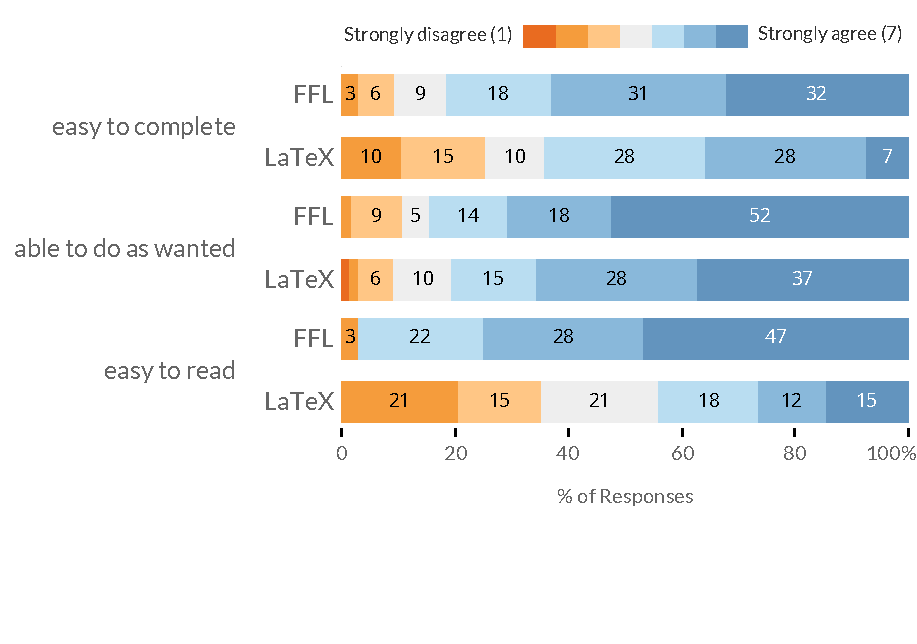
\includegraphics[width=\linewidth]{figures/Responses.pdf}
    \vspace{-2.5em}
    \caption{Self-reported ease for timed tasks. On the whole, participants reported greater ease with FFL than with LaTeX. \normalfont Data comes from responses when participants were asked to indicate agreement (from "strongly disagree" (1) to "strongly agree" (7)) with the statement in the left column of the bar chart. Numbers indicate percentage of total responses relative to the row. \zed{Per-row medians and arithmetic means appear in Tables \ref{tab:ease_table}--\ref{tab:ease_to_read_table}}.}
    \Description{Stacked bar chart of self-reported ease for timed tasks (on a 7-point Likert scale). The three dimensions of ease are “easy to complete”, “able to do as wanted” and “easy to read.” Greater ease is reported with FFL for all three; this difference is slight for “able to do as wanted” and pronounced for “easy to complete” and “easy to read.”}
    \label{fig:responses}
\end{figure}

\subsubsection{Ease}\label{sec:ease}

Participants reported significantly higher ease completing tasks with FFL than with LaTeX ($F=16$, $p=6\times10^{-4}$). On a 7-point Likert scale, participants reported \zed{a median score of 7.0}, versus \zed{6.0} with LaTeX (Figure~\ref{fig:responses}). Models fit on subsets of tasks showed the difference in ease to be significant for editing tasks E1 \& 2 ($F=19$, $p=2\times10^{-4}$), but not tasks C1 \& 2 ($p\approx1$).

Additional questions on the questionnaire indicate aspects of FFL that might have led to greater ease. Following the editing tasks E1 \& 2, participants reported significantly greater ease in reading augmentation code (Figure~\ref{fig:responses}) in FFL than with LaTeX ($F=23$, $p=6\times10^{-5}$). In the retrospective questionnaire, participants compared the ease of using FFL to LaTeX for a variety of primitive augmentation operations (Figure~\ref{fig:eos1}), reporting greater ease with FFL for coloring parts of formulas ($W=7$, $p<0.002$, \zed{mdn. 5.0 vs. 4.0}), labeling parts of formulas ($W=0$, $p<0.002$, \zed{mdn. 5.0 vs. 4.0}), and applying the style to multiple parts of the formulas ($W=24$, $p<0.002$, \zed{mdn. 5.0 vs. 2.0}), on a 1--5 scale.

% \begin{center}
\begin{figure}
    \centering
    \vspace{-.5ex}
    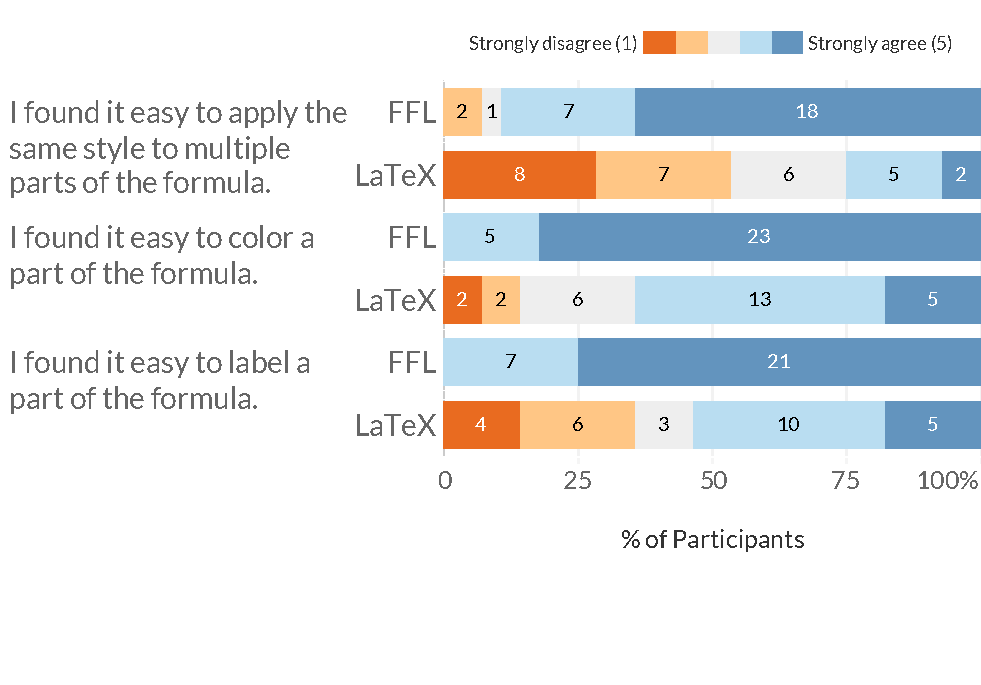
\includegraphics[width=\linewidth]{figures/EOS-1.pdf}
    \vspace{-2.5em}
    \caption{Ease-of-use ratings in retrospective questionnaire. \normalfont Ease was reported on three dimensions for both FFL and LaTeX (shown in the leftmost labels on the bar chart). % \normalfont Participants participants were asked to rate on a scale from "strongly disagree" (1) to "strongly agree" (5) on their agreement with the statement on the left after each task.
    \vspace{-1ex}}\Description{Stacked bar chart of ease-of-use responses in retrospective questionnaire, for three questions asked on a 5-point Likert Scale. The three questions are, “I found it easy to apply the same style to multiple parts of the formula,” “I found it easy to color a part of the formula,” and “I found it easy to label a part of the formula.” A majority of participants “strongly agreed” that FFL made tasks easy in these three ways. Agreement was weaker for LaTeX; with LaTeX, for applying the same style to multiple parts of the formula, 7 / 28 participants reported agreement (either a 4 or 5 out of 5); for coloring a part of the formula, 18 / 28; and for labeling a part of the formula 15 / 28.}
    \label{fig:eos1}
\end{figure}
% \end{center}
% % Possibility of real-life usage
% Some participants' responses to the questionnaires also indicate their interest in using FFL in real-life practice. 
% \begin{itemize}
%     \item “I would use it to make my smaller projects prettier. \LaTeX\ takes a lot of typing and learning even though it might be more powerful” (P4) % Jiening: should I leave the second sentence out?
%     \item “Great idea for this styling option! Looking forward to see it in the real application!” (P12)
%     \item “When can I get this tool installed as an extension on Overleaf?” (P13)
%     \item "I think it's probably best to use both at the same time" ("Both" here refer to \LaTeX\ and FFL). (P19) 
% \end{itemize}

\subsubsection{Differences in success}
% \subsubsection{The Effect of Participant's Backgrounds}

% \andrew{@Andrew: simplify this section}
%Learning barriers

While on the whole participants reported high levels of comfort with LaTeX in the introductory questionnaire, there was still considerable individual variation in comfort with both LaTeX and CSS. When we fit our model to take background factors into account,\footnote{When fitting a model with background factors as fixed effects, we remove the random effect of participant ID.} we observed years of experience of LaTeX as a significant predictor of task speed ($F=10$, $p=5\times10^{-5}$), with interface becoming insignificant ($F=5.4$, $p=.1$). For the creation tasks alone, years of experience with LaTeX is not significant  ($p=.3$). For the editing tasks, years of experience is significant ($F=10$, $p=3\times10^{-4}$), and interface remains a significant effect ($F=27$, $p=6\times10^{-5}$). Other background factors such as self-reported comfort with LaTeX or CSS were not significant predictors. Overall, additional years of experience of LaTeX reduced task completion times, though the trends vary considerably when broken down by task and interface pair.

% Although we considered participants as a random effect in our previous modeling, this prompted us also to investigate the effect that participants' background might have on the measurements. This is only true in regards to task completion times. In fact, if we model over all tasks with background questions included as factors in place of participant as random effect, participants' (ranges of) years of experience using LaTeX, encoded as an ordinal, becomes the most significant factor ($F\approx10.37$, $p\approx5.21\times10^{-5}$), and interface becomes much less so ($F\approx5.38$, $p\approx0.113$).

% This does affect both task groups differently. Looking at the two task groups individually, we again see no significant factor as expected in tasks A \& B, although it might be interesting to note that this becomes the only factor with $p<1$ ($p\approx0.328$), while in C \& D, it still has notable significance ($F\approx10.08$, $p\approx3.25\times10^{-4}$), but it does not greatly diminish the effect of the interface ($F\approx26.84$, $p\approx5.65\times10^{5}$). This does not change our general observation that FFL performs better in the more complex group of tasks in our lab study.

% Curiously, years of experience with \LaTeX\ seem to be the only factor that has this effect, while responses to similar questions such as frequency using \LaTeX\ or self-reported comfort with \LaTeX\ or CSS do not.

\subsubsection{Interpretation}

In summary, participants completed tasks about as often with FFL and LaTeX. FFL led to quicker completion, with less difficulty. Post-hoc tests showed the effect to be significant for editing tasks E1 \& 2, but not creation tasks C1 \& 2. We explain this discrepancy with two observations. 

First, E1 \& 2 were performed after C1 \& 2. Some participants reported an initial learning curve with FFL, or encountered gaps or misconceptions regarding FFL during the first pair of tasks. These gaps and misconceptions were sometimes resolved by the time they began the second pair of tasks. Learning effects may provide as a partial explanation: among 33 participants, our observation notes showed 23 participants making 35 critical mistakes \zed{(i.e., input that resulted in compilation errors or incorrect outputs)} in C1 \& 2, reduced to 18 participants making 23 mistakes in E1 \& 2.

Second, E1 \& 2 required participants to work with considerably more complex and denser markup along with some augmentation already integrated to begin with. E1 \& 2 reflect a setting where a formula has been augmented and the authors wish to experiment with alternative designs. We interpret this effect to indicate that FFL manifests more value as augmentation markup becomes larger \zed{and the presence of existing augmentation code in the editing tasks served as a scaffold in case of unfamiliarity with FFL's syntax}; in the LaTeX baseline, this results in the markup languages becoming increasingly tangled and difficult to evolve, as discussed in greater detail in the next section.

% \subsubsection{Ease/"It was easy to complete the task." (1-7)}\ \\[1ex]
% \scalebox{0.93}{
%     \begin{tabular}{l|r r r r r}
%         Avg. Score (1-7) & Task A & Task B & Task C & Task D & Open Task \\\hline
%         FFL     &5.47&5.31&6.38&5.44&6.30\\
%         \LaTeX  &5.00&5.24&5.13&3.61&N/A
%     \end{tabular}
% }\\[1ex]

% As data shown in Table \ref{tab: ease_table} in \ref{sec: result_table}, participants generally also find it easier to complete the tasks in FFL compared to in \LaTeX\ in both models ($F\approx15.96$, $p\approx5.89\times10^{-4}$), similar to the above with the response variable being the only difference, with no other major contending factor, with FFL averaging at $5.867$ on the 1-7 scale and \LaTeX\ at $4.716$, as also seen in Figure \ref{fig:responses}, again with tasks C and D driving the difference ($F\approx19.43$, $p\approx2.15\times10^{-4}$), and no significance ($p\approx1$) again in tasks A and B, which suggests again FFL performs similarly to \LaTeX\ in simple tasks but outperforms \LaTeX\ in more complex augmentation tasks. Note that the overall aggregation includes the open task, which we are not able to test against the \LaTeX\ baseline, although we can see that participants generally respond positively to the statement in regards to this task.

\subsection{Effect of FFL on authoring experience}

In this section, we review observations, interviews, and questionnaire data to arrive at a comprehensive understanding of how FFL supports, and in some cases works against, the experience of formula augmentation. Overall, participants found FFL's ``core'' features useful (Figure~\ref{fig:features_use}). This section introduces strengths and shortcomings of FFL in terms of the cognitive dimensions of notation~\cite{ref:blackwell2003notational}, a framework used in programming language design to \zed{examine and discuss} the effect of language design choices.

% \begin{center}
\begin{figure}
    \centering
    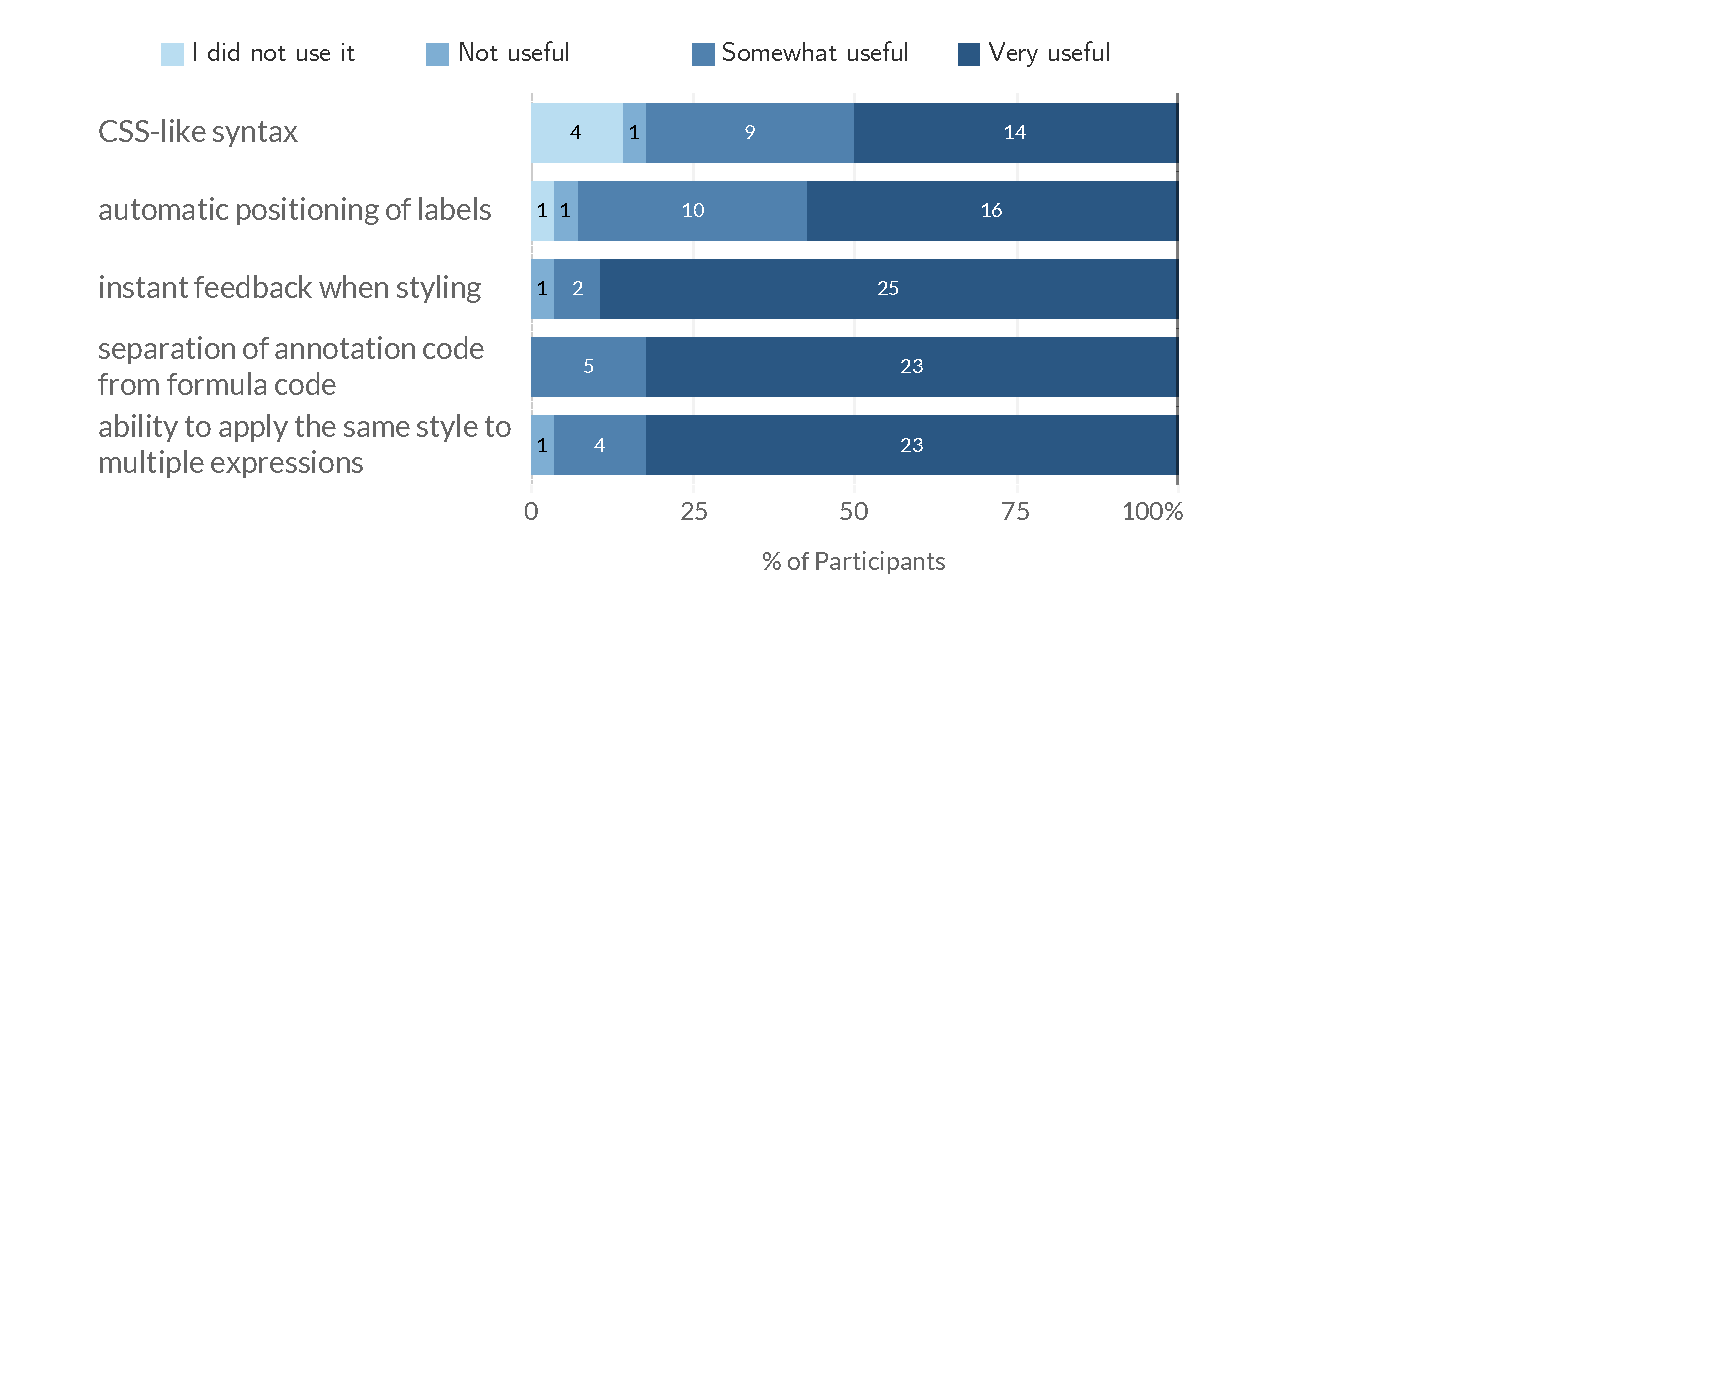
\includegraphics[width=\linewidth]{figures/Useful.pdf}
    \Description{Stacked bar chart of usefulness of 5 features (on a 4-point scale, including “I did not use it,” “not useful,” “somewhat useful,” and “very useful”). The five features are “CSS-like syntax,” “automatic positioning of labels,” “instant feedback when styling,” “separation of annotation code from formula code,” and “the ability to apply the same style to multiple expressions.” For all features except for “CSS-like syntax,” a majority of participants reported “very useful.” The vast majority of participants found “instant feedback,” “separation of annotation code from formula code,” and “the ability to apply the same style to multiple expressions” very useful. 14/28 participants found CSS-like syntax very useful, and 9/28 participants found it somewhat useful.}
    \caption{Usefulness of features. \normalfont Shown are participants reponses to the question ``How useful was \emph{[feature]} when you used FFL to augment math formulae?''% \normalfont (``I did not use it''/``Not useful''/``Somewhat useful''/``Very useful'').
    }
    \label{fig:features_use}
\end{figure}
% \end{center}

% while identifying  some aspects of the toolkit FFL environment might have created friction.

% General praise:

% It improved readability with fewer layers of braces involved which makes FFL ``a really cool tool''(P14). 

\subsubsection{Strengths} FFL improved the authoring experience as follows:

\paragraph{Viscosity}
FFL reduced the number of actions required to accomplish some goals. This was most clear when participants edited augmentations for multiple expressions at once. Participants frequently expressed appreciation for the ability to make cross-cutting changes with a single style specification (5), and wished for a similar capability for LaTeX (4). Making cross-cutting changes was described as more ``efficient'' (P4) and ``easier'' (P12, P24) with FFL. \zed{All but one} participant described the ability to apply one style to multiple expressions as very useful (Figure~\ref{fig:features_use}).

% \andrew{Mention one participant's quote about overriding colors here?} Zed: leaving it out given the number of questions otherwise

% The improved ability to make cross-cutting changes was also endorsed by participants (P4, P12, P24, P28, P32) and is favored over \LaTeX\ where 4 participants wished for similar capability. This feature in FFL enabled participants to apply the same styles to multiple expressions in a more "efficient" (P4) and "easier" (P12, P24) way. In particular, P32 mentioned that wildcards is a helpful factor in styling similar patterns.

% P12 stated that they "like that you can overwrite colors" when they found the overriding behavior of FFL (later overrides prior) intuitive and their goals didn't involve anything that couldn't be easily done by overwriting. P30 also mentioned in the interview that \begin{quote}

\paragraph{Hard mental operations}

FFL made it easier for participants to orient themselves to augmentation markup. LaTeX was the less preferred choice for reading markup (Figure~\ref{fig:responses}). LaTeX was described as difficult to read (16) and used complex or unintuitive syntax (6). The association of augmentations with expressions is difficult to understand due to the dependence on copious numbers of nested braces to associate them (14). Reading LaTeX was therefore described as ``holding a lot of moving pieces in my mind'' (P18), where ``it is a nightmare to look for what I am editing'' (P13). Reading challenges arose when participants had difficulty identifying expressions to which LaTeX commands applied (2), mapping from parts of the rendered formula to the corresponding LaTeX (5), reading and editing the markup (3), and pinpointing sources of errors (2).

% When formulas and styles were interleaved\ldots{}

 % \begin{quote}
% ``it will impede my reading\ldots{} they will just be like a cluster of everything. That's so hard to find which parts belong[s] to which part. So it's not really readable or eligible to me.'' (P8)
% \end{quote}

In comparison, FFL seemed easier to read---we rarely heard similar criticisms levied against FFL. 16 participants explicitly mentioned their appreciation for the separation of formula markup from augmentation markup; this division was called a ``big advantage'' and ``very powerful'' (P13). The separation of annotation code from formula code was reported as ``very useful'' by the vast majority of participants in the retrospective questionnaire, and ``somewhat useful'' by all remaining participants. Participants rated the readability of FFL significantly higher than LaTeX (Section~\ref{sec:ease}).

% FFL addressed this problem of everything ``jammed'' together with the separation of augmentation code from formula code, which 16 participants found helpful.  
% \begin{quote}
% ``[in \LaTeX] \dots you go ahead and make a bunch of edits but then when you come back to make edits to the part of the code already wrote, it is a nightmare looking for what I am editing. I wanna wrote my stats homework and it involved complex formulas, I read the whole thing and later I found out I didn't include a square sign to a variable. I'm going to change it and I spent 5 minutes just looking for every instance of that variable in that long equation and that was a nightmare. So that was the main problem for \LaTeX. [FFL]'s separating style has been a  big advantage and also the ability to apply a single change to the same variable. That is very powerful. I like that.'' (P13)
% \end{quote}

% Particularly, participants felt that it was difficult to keep track of all the styling code in \LaTeX\ (1), identify the scope of \LaTeX\ command arguments (2), identify the parts of maths markup matching the rendered formula (5), navigate to and locate the precise parts to edit (2), read and edit codes by others (3), locate errors in the code (2), and read the non-style content with styling codes mixed in (1). \begin{quote}
% ``If I put too much styling text next to the actual content, it will impede my reading of what I actually have over there. So, In the end, they will just be like a cluster of everything. That's so hard to find which parts belong to which part. So it's not really readable or eligible to me.'' (P8)
% \end{quote}
% In addition, 6 participants showed a desire for more space and separations within the \LaTeX\ formula markup. 

% \begin{quote}``[with LaTeX,] styling is incorporated into the text editor[, which] requires holding a lot of moving pieces in my mind. When there's a lot of text \& formatting it would get much hard, but it was fairly easy because the formula and coloring was not too extensive'' (P18)
% \end{quote}

% In more complex tasks, participants faced more challenges with \LaTeX\ editing, including distraction from normal editing objective due to the dense code involving both styling and formula (3), complex and unintuitive syntax (6) such as complicated commands (P6, P8) as well as too many nested braces (14).

% theme: messy markup
% Notably, 16 participants' responses complained about the readability of \LaTeX, which was sometimes described as ``messy'' (P7). 

\paragraph{Error proneness}

FFL removed a class of errors with its approach to associating expressions with augmentations. As mentioned in prior work~\cite{ref:head2022math}, one challenge of using LaTeX to augment formulas is to use braces correctly to associate augmentations with expressions. Participants described braces as ``annoying'' (P28), finding it difficult to find matching pairs of braces (6), and desiring the ability to find out which braces are redundant or missing (2). Braces were the most common kind of error we observed: at least some participants made a bracing error for each task (8 participants for task C1; 2 for C2; 6 for E1; and 8 for E2). Participants also encountered issues with using \texttt{\textbackslash{}def} correctly, writing arguments to commands in the right order, and other LaTeX compilation errors. As noted by participants, FFL did not see these difficulties due to its approach to associating augmentations with expressions (2).

% Managing braces also relates to resulted in hard mental operations.

% Braces is a particular ``annoying'' problem (P28). Participants found it difficult to find matching braces (6), and \LaTeX\ is not able to suggest which braces are redundant or missing (2).

% Easy to edit
% FFL avoids the problem of requiring using nested braces by design. Two participants (P12, P30) considered using FFL to make editing easier due to less usage of braces. This advantage is also often used in conjunction with the overriding behavior of styles.
% P12 stated that they "like that you can overwrite colors" when they found the overriding behavior of FFL (later overrides prior) intuitive and their goals didn't involve anything that couldn't be easily done by overwriting. P30 also mentioned in the interview that \begin{quote}
% "\dots the fact that you don't use so many brackets is very useful because now you won't make mistakes. It helps you make it very quick when you're trying to make a change; it's much much quicker compared to having to slowly read through the passage and see where you need to annotate and make changes." 
% \end{quote} 

\paragraph{Closeness of mapping}

In several situations, FFL provided a close mapping to the ways participants could envision expressing augmentations. Two participants described that the metaphor of CSS, including its use of selectors and attributes, was ``intuitive.'' The design of selectors allowed participants to indicate which expressions they wished to augment by selecting, and then copying and pasting, those expressions from the formula into their FFL specification (2). When asked to indicate the degree to which FFL ``did what I expected to,'' all but 2 participants agreed, and over half of participants strongly agreed.

On the whole, participants developed comfort with a large number of primitives in a short amount of time. By the time they performed the exploratory authoring task, participants had developed enough comfort with the language that they frequently made use of color (24), labels with leader lines (19), and labels with extent markers (11). These augmentations made use of myriad language features, including single character wildcards (15), sequence wildcards (15), unions (11), and the adjustment of label positions (9). See Appendix Section~\ref{sec: open_task_image} for examples.

% \paragraph{"[FFL] did what I expected it to." (1-5)} We again report a generally positive response, as seen in Figure \ref{fig:expectation}. While there are limitations with the prototype, as we will discuss later, it is promising to see that FFL meets the expectation of participants. Note that this one and all metrics that follows do not have paired measurements against the \LaTeX\ baseline.

% Participants with prior knowledge of CSS felt that FFL was ``intuitive'' for CSS users (P16, P30), with the selectors and attributes being ``intuitive'' (P16).

% We noticed participants' general appreciation for the separation of annotation code from formula code. 16 participants mentioned the helpfulness of separating formula and styling. While the design of separation in FFL enhanced the readability as discussed in 7.1.4, it also made styling easier because it was easier to copy, paste, and apply similar styling code blocks to different selectors in FFL compared to the case in \LaTeX\ where people had to further edit the content inside the braces after pasting the copied codes (P30, P4). \begin{quote}
% “Easy to copy and paste styling and make changes in Tool X [FFL] while in Tool Y [\LaTeX] you need to slowly read through everything” (P30)
% \end{quote}


\paragraph{Progressive evaluation}

The favorite feature of FFL was the instant feedback supported by the FFL runtime. More participants described this feature as ``very useful'' than any other feature. 7 participants explicitly indicated their appreciation for instant feedback. In contrast, the LaTeX toolset required slower compilation of the document to see the effect of one's changes to the markup (2), which was described as ``not very convenient'' (P21).

% The feature of instant rendering was mentioned as their preference by 7 participants (P7, P16, P21, P22, P29, P19, P28). Compared to \LaTeX\ which needs to ``click compile to see the changes every time'' (P21) which is ``not very convenient'' (P21) and miss the ability to ``see the changes right away'' (P22), participants generally favored the instant feedback of FFL.

% \begin{quote}
%      `I really like Tool X [FFL] compared to the other one [\LaTeX] because I like the intermediate feedback, because I can change and compare.'' (P22)
% \end{quote}

% \begin{quote}
%     ``I liked how for X [FFL] you have instant feedback. I did not need to constantly refresh every compile of the page as I need to do in Overleaf.'' (P28)
% \end{quote}

\subsubsection{Shortcomings}\label{sec:shortcomings} While FFL improved the experience of authoring formulas in numerous ways, it also introduced new challenges meriting new solutions to design and training:

\paragraph{Closeness of mapping}
FFL was not without a learning curve. Some participants found aspects of the CSS-like syntax challenging (8); this is in part because participants generally had low self-reported comfort with CSS (Section \ref{study-participants}). Participants also expressed discomfort with the \texttt{glob} syntax~\cite{UnixMan} for wildcards (1), and other aspects of LaTeX's math mode (5). These experiences serve as a reminder that FFL expects familiarity with CSS, glob, and LaTeX. We expect many authors seeking to use FFL in web documents would have this experience; though FFL still imposes a threshold to entry. An additional indicator of a learning curve is that 8 participants reviewed the cheat sheet before beginning their first task with FFL, suggesting that the tutorial was not enough to internalize the syntax. Similar challenges were observed for the LaTeX baseline, with participants forgetting commands taught in the tutorial (3) or failing to properly use commands from the cheat sheet (3).

While participants largely succeeded in selecting expressions with the selector syntax, several participants desired support for direct selection through mouse interaction with the formula (3). Similarly, participants desired the ability to highlight expressions corresponding to a selector (3). Participants also desired code generation (1) and no-code features (2), where style code could be partially or completely generated for the author. Direct selection features are beyond the scope of a language design, though they might serve as useful additions to an editing environment.


% Notably, 5 participants wanted to select multiple things together into a ``custom class'' and apply styles to the class, which would be easier to organize and modify the styles in bulk. 

% \begin{quote}
% ``there are times when I feel that in CSS, there is something called a class, and I can just apply the class to multiple things. So, I want this thing where I have a class, right? And the class I list for attributes and that class I can directly add to different things rather than selecting multiple things and giving them brackets. I want to be able to select like add one class to everything else and wrap these elements into one class and apply attributes to the class.''  (P20)
% \end{quote}

% \begin{quote}
% ``[one improvement would] be able to select by keys (like select all attributes involving a color tag etc., and apply a change to the whole group)'' (P13)
% \end{quote}

\paragraph{Error proneness}

FFL removed some classes of errors, though they introduced friction for others. The current runtime provides only very limited support for error tolerance, reporting, and recovery. 6 participants introduced typos and had difficulty understanding why their augmentation markup was not working as intended when they failed to notice those typos.
% \zed{, where the rendered formula stopped updating and the interface only reported a nondescript error.} \andrew{Is this true for all of the 6 participants? Maybe we should soften this to instead say that the current error reporting interface was insufficient to help them identify and fix the errors} \andrew{I think to address reviewer feedback, we should instead describe error reporting capabilities in the way that we do in the rebuttal, when describing the live editor system. Here, the information is easy to miss.}
Some of these typos arose from challenges related to ``closeness of mapping''---several participants used incorrect delimiters that perhaps best reflected a lack of familiarity with the base CSS syntax. 3 participants wished that FFL continued to render live even when errors were present in the markup. For these reasons, participants desired numerous standard editor affordances that assist in reducing errors, including autocomplete (7), syntax highlighting (2), and templates (3).

% Currently, FFL's editing environment is missing common editor features which participants expect (13) out of habit with common IDE interaction patterns such as trying \texttt{Ctrl-F} (1) and \texttt{Ctrl-S} (2) when editing. Among the expected features are auto-complete (7), smart indentation (2), support for templates (3), syntax highlighting (2), color palette (1), more ``undo'' history checking (1), search (1), and multi-file support (1), some among which would also assist in identifying slips.

% they did introduce others; participants 

% While participants were generally able to achieve their goals with FFL, they did sometimes encounter slips while editing. One of challenges was insufficient support for identifying slips. In \LaTeX, 3 participants showed a negative attitude towards the fact that the preview page will stop rendering if there is an error that is ``annoying'' (P1). In FFL, while the preview still renders with typos and errors, 3 participants complained that keywords are sensitive to typos in FFL, but FFL currently does not support reporting unrecognized properties. 6 participants wondered why their input styling didn't work when they failed to notice typos.

\paragraph{Visibility}
Any sufficiently complex language contains constructs users are unaware of. We observed several such constructs for FFL that were either undiscoverable, or poorly suited once discovered.

First, participants expressed confusion around scoping augmentations. The default behavior of the FFL runtime is to apply selectors globally across an entire document. What should an author do when they wish for their augmentation rules to apply to only a single expression, formula, or single passage? Several authors had this specific question (8). The current solutions in FFL are: (1) the \texttt{intersect} command; (2) an \texttt{:nth} selector that selects an indexed occurrence; (3) creating an indexable group in the formula markup by adding brackets around it; (4) using style overriding (i.e., using one rule to style all expressions, and a second rule to revert it for some subset of those expressions). These features were largely unused, perhaps due to issues of discoverability or learnability. At least 2 participants expressed some confusion with overriding.

Second, participants desired more influence over the appearance of labels, including label size (4), color (3), and font weight (3). While the \texttt{.ffl-label} class is applied to all labels for just this purpose, participants were not often aware of it. These undiscovered features represent opportunities to either increase visibility, or redesign constructs to be easier to guess.

\paragraph{Expressiveness}
Expressiveness is not a cognitive dimension of notation, though we discuss it here as a catchall for controls participants desired that FFL did not provide. One often-desired feature was the ability to assign a single label to multiple expressions simultaneously. For example, in the exploratory task, participants often wanted to create one label for ``slope'' and connect it via leader lines to all four $\beta$ terms in the formula (9). The default behavior of FFL is to assign a label to only the first matched expression in a formula. As one participant noted, this made the behavior of FFL inconsistent, because style rules applied to all matching expressions, while labels applied to only the first matched expression (P23). Several participants wished for different behavior from the automatic label layout algorithm (4), and desired the ability to fine-tune label layout beyond FFL's current capabilities (3).

% Third, participants desired more influence over the appearance and layout of labels. Participants desired the ability to change label size (4), label color (3), and font weight of the label text (3). While we already attach a \texttt{ffl-label} class to the elements, more design needs to be considered in order to satisfy the needs of authors.

% 9 participants want to assign a single label to multiple expressions simultaneously. More specifically, they wanted to label all the $\beta$ slope terms in the formula of linear regression with the selector \texttt{\$\textbackslash beta\_*\$}. By default, the label is only attached to the first $\beta_0$ term, despite the fact that all $\beta$'s with subscripts are technically matched by the selector. They expected to have one single label linked to all $\beta$ terms instead, which ``may be helpful'' (P21). 
% This is a design decision we made in order to achieve ``pretty defaults.'' However, this unexpected behavior leads to inconsistency between the color and label properties. P23 wondered why the label only applies to the first selection but the color can apply to all; P27  `` expect it [the label] to be on all of [the terms].'' According to P6, “the label part can be better to add multiple lines to signal label”, which may make the formula more understandable, although how this should be achieved might still require further design.

% Automatic positioning of labels could be improved by enabling more customization as well. We notice a few responses (4) show dissatisfaction from the participants about the label auto-positioning because it placed the labels in an unexpected location, as labels are shifted to avoid overlap with each other in the prototype. Specifically, P27 mentioned that ``Sometimes it pushes [the labels] the way I didn’t want it to''; By P16, \begin{quote}
% `` I didn't know that there was limited space in a particular "box", which was causing the flux [label text] line to be bent. The auto-placement is meant to avoid overlap, but was not obvious. Especially since when I used it before, it went straight down. '' (P16)
% \end{quote}

% messy syntax of latex: difficult to edit + braces

% \subsubsection{Readability/"I found it easy to read the styling code/specification" (1-7)}
% \begin{center}
%     \vspace{-1em}
%     \scalebox{0.93}{
%         \begin{tabular}{l|r r r r r}
%             Avg. Score (1-7) & Task C & Task D \\\hline
%             FFL     &6.25&6.00\\
%             \LaTeX  &5.06&3.61
%         \end{tabular}
%     }    
% \end{center}
% This statement only applies to tasks C and D, as these are the only tasks where we have provided starting styling code. From Table \ref{tab: ease_to_read_table} in \ref{sec: result_table} we see FFL outperforming \LaTeX\ by a notable margin ($F\approx22.98$, $p\approx5.83\times10^{-05}$) in precieved readability.

% \andrew{Can we expand on this any more? Most of this subsection talks about how difficult it was to use LaTeX; I wonder if we can shift the focus more onto FFL.}

% \subsection{Feature usage}
% For the end of study questions (Figure \ref{fig:eos1}) where we asked participants to compare their impressions between the two interfaces, we perform Wilcoxon signed-rank tests on the 1-5 Likert scale responses.

% We also asked participants ``How useful was \dots when you used FFL to augment math formulae?'' As can be seen in Figure \ref{fig:features_use}, all major features surveyed saw usage by most participants and received largely positive responses.
% \begin{figure}[H]
%     \centering
%     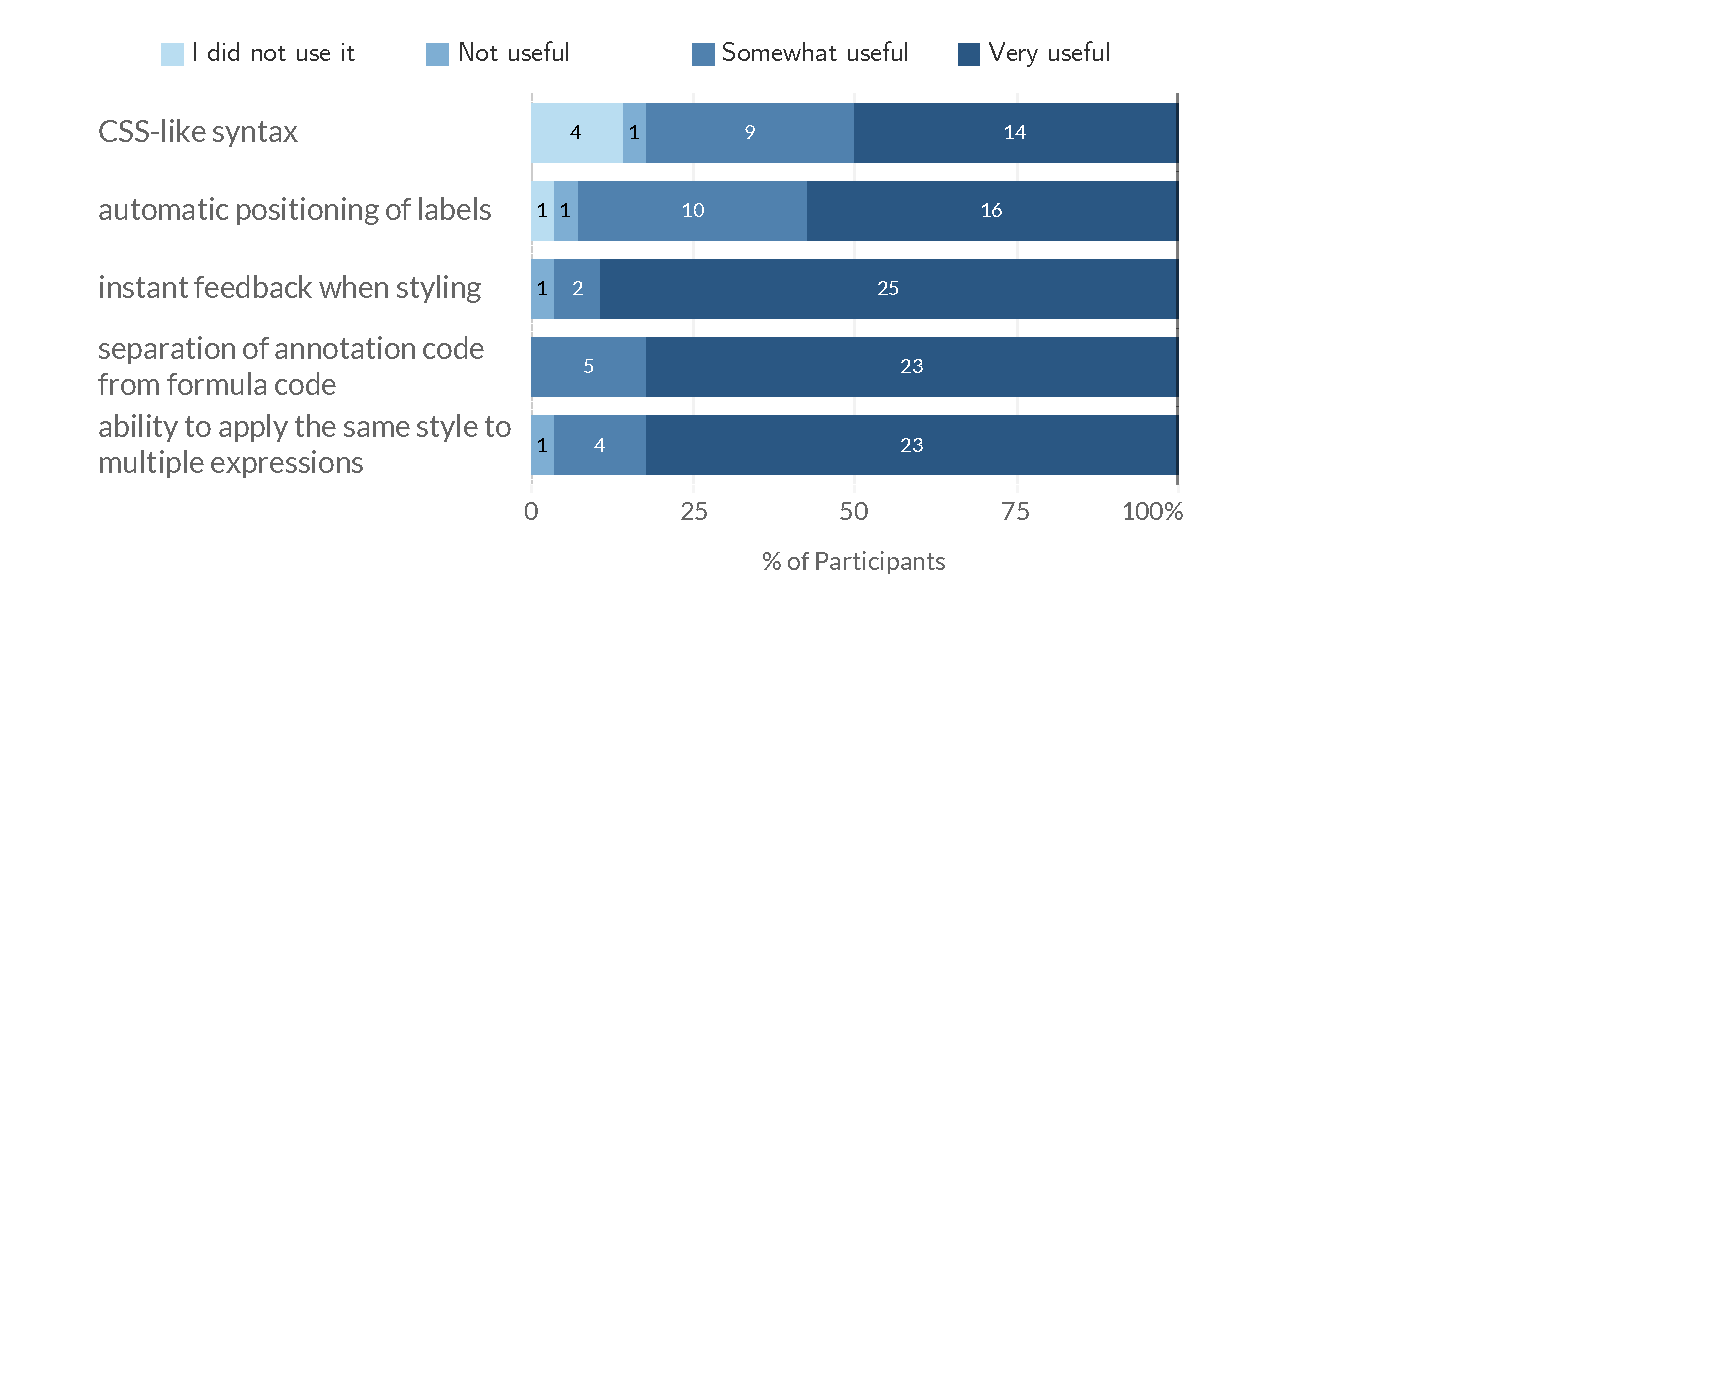
\includegraphics[width=\linewidth]{figures/Useful.pdf}
%     \caption{``How useful was \dots when you used FFL to augment math formulae?'' \normalfont (``I did not use it''/``Not useful''/``Somewhat useful''/``Very useful'').}
%     \label{fig:features_use}
% \end{figure}
% The most ``I did not use it'' response occured with regards to ``CSS-like syntax,'' this is likely due to the fact that a few of the participants being unaware of CSS, as it is not possible to avoid it in FFL, similarly with ``automatic positioning of labels,'' which might indicate that participants might not have noticed the behavior. Otherwise, the participants were able to successfully learn and utilize the introduced features.
 
% This observation is also supplemented by the number of participants that we observed using certain features in the exploratory task,\\[1ex]
% \begin{tabularx}{\linewidth}{X r}
%     \textbf{Feature}&\textbf{\# of Participants}\\\hline
%     Use of colors		                & 24 \\
%     Use of line labels		            & 19 \\
%     Use of wildcard (?)	                & 15 \\
%     Use of wildcard (*)	                & 15 \\
%     Connectives (“,”)	                & 11 \\
%     Assignment of color to text spans\footnote{refers to using a regular CSS class selector to select added \texttt{span} tags in order to style text elements, only taught to participant if asked}
%                                         & 11 \\
%     Use of extent labels		        & 9  \\
%     Adjustment of label positions		& 9  \\
% \end{tabularx}\\[1ex]
% Interestingly, the adjustment of labels are not used as common as some other features, despite it being required to complete most tasks.

% \subsection{Desired Improvements}\label{sec:improvements}
% Our study also collected feedback to help crystallize how tools like FFL could be improved in the future to better support authors in augmenting formulas.

% \andrew{Lead with scoping and power features (there are the ones that will be most informative to those in research who want to explore novel ways to improve FFL-like languages and runtimes), end with support for identifying slips and editor support.}

%\paragraph{difficult to organize when codes get long} 

% \subsubsection{More Powerful Features}
% Despite all the potential improvements on existing problems, participants also expressed a desire for more powerful features in FFL. 

% \paragraph{Label customization (16).}
% 9 participants want to assign a single label to multiple expressions simultaneously. More specifically, they wanted to label all the $\beta$ slope terms in the formula of linear regression with the selector \texttt{\$\textbackslash beta\_*\$}. By default, the label is only attached to the first $\beta_0$ term, despite the fact that all $\beta$'s with subscripts are technically matched by the selector. They expected to have one single label linked to all $\beta$ terms instead, which ``may be helpful'' (P21). 
% This is a design decision we made in order to achieve ``pretty defaults.'' However, this unexpected behavior leads to inconsistency between the color and label properties. P23 wondered why the label only applies to the first selection but the color can apply to all; P27  `` expect it [the label] to be on all of [the terms].'' According to P6, “the label part can be better to add multiple lines to signal label”, which may make the formula more understandable, although how this should be achieved might still require further design.

% Automatic positioning of labels could be improved by enabling more customization as well. We notice a few responses (4) show dissatisfaction from the participants about the label auto-positioning because it placed the labels in an unexpected location, as labels are shifted to avoid overlap with each other in the prototype. Specifically, P27 mentioned that ``Sometimes it pushes [the labels] the way I didn’t want it to''; By P16, \begin{quote}
% `` I didn't know that there was limited space in a particular "box", which was causing the flux [label text] line to be bent. The auto-placement is meant to avoid overlap, but was not obvious. Especially since when I used it before, it went straight down. '' (P16)
% \end{quote}

% 3 participants also indicated the desire for manual control of the label positions, which can only be specified \texttt{above} or \texttt{below} currently. Other types of label style customization are also mentioned, such as label size (4), label color (3), and font weight of the label text (3). While we already attach a \texttt{ffl-label} class to the elements, more design needs to be considered in order to satisfy the needs of authors.

% \paragraph{Advanced selection support (11).} 3 participants mentioned that it would be easier to select a portion of the formulae through a point-and-click style interface. One mentioned that “it would also be nice if we can drag elements [in the rendered math formula] on the preview and change the code that way.” (P13) 3 participants expected the selected portion can be highlighted in the original formula code. Notably, 5 participants wanted to select multiple things together into a ``custom class'' and apply styles to the class, which would be easier to organize and modify the styles in bulk. 

% \begin{quote}
% ``there are times when I feel that in CSS, there is something called a class, and I can just apply the class to multiple things. So, I want this thing where I have a class, right? And the class I list for attributes and that class I can directly add to different things rather than selecting multiple things and giving them brackets. I want to be able to select like add one class to everything else and wrap these elements into one class and apply attributes to the class.''  (P20)
% \end{quote}

% \begin{quote}
% ``[one improvement would] be able to select by keys (like select all attributes involving a color tag etc., and apply a change to the whole group)'' (P13)
% \end{quote}

% \paragraph{Code generation or no-code augmentation (5).}
% \begin{quote}
% “If clicking character and some of the standard styling text could be auto-generate, it will be much easier” (P8)
% \end{quote}
% \begin{quote}
% “If there's a way to do it without any coding involved then it would be easier for people who are not familiar with CSS” (P1)
% \end{quote}
% \begin{quote}
%  "If there is a button I can just click to select the style I need it would probably be easier" (P1).
% \end{quote}

% \paragraph{Easier coloring of document text (1).}
 % For coloring markdown text, we taught participants to use \texttt{<span>} tags with CSS classes to mark the text they want to select and put \texttt{*.class-name} in the styling code block to select and color the markdown text. P27 expected an alternative way which could be a quicker action or snippet.

% \subsubsection{More support for identifying slips}
% While participants were generally able to achieve their goals with FFL, they did sometimes encounter slips while editing. One of challenges was insufficient support for identifying slips. In \LaTeX, 3 participants showed a negative attitude towards the fact that the preview page will stop rendering if there is an error that is ``annoying'' (P1). In FFL, while the preview still renders with typos and errors, 3 participants complained that keywords are sensitive to typos in FFL, but FFL currently does not support reporting unrecognized properties. 6 participants wondered why their input styling didn't work when they failed to notice typos.

% A more detailed error reporting mechanism was also expected by 3 participants. For example, it was suggested that FFL "maybe show an error message when people forget to add \texttt{;}" (P3).

% \subsubsection{Editor support}
% Currently, FFL's editing environment is missing common editor features which participants expect (13) out of habit with common IDE interaction patterns such as trying \texttt{Ctrl-F} (1) and \texttt{Ctrl-S} (2) when editing. Among the expected features are auto-complete (7), smart indentation (2), support for templates (3), syntax highlighting (2), color palette (1), more ``undo'' history checking (1), search (1), and multi-file support (1), some among which would also assist in identifying slips.


% One set of challenges was caused by the fact that some participants were not familiar with the CSS-style syntax. For some participants, the necessity to include semicolons after each property posed difficulties, with 5 participants preferring another syntax for delimiting properties (like spaces or commas), and 6 forgetting to use a semicolon at some point. 3 participants made slips related to other delimiters (like inserting ``:'' where it need not be, or using a ``='' in place of a ``:'').

% Another class of slips related to selections. Participants made a variety of individual slips, including forgetting to escape Greek letters (1), forgetting to use \texttt{\$} signs to mark LaTeX selectors (1), and doubling the dollar signs (1). P23 described confusion around selecting particularly long expressions, noting that it felt uncomfortable to select longer expressions by writing the expression literally in the selector.



